\subsection{Language coverage}

The first statistic consists of determining how much of the language is covered by the $k$ most used words. The result is shown in figure \ref{coverage_figure}. We could see that, with the same amount of words, we cover less and less of the language from 1840 to 1995.

\begin{figure}[H]
	\centering
    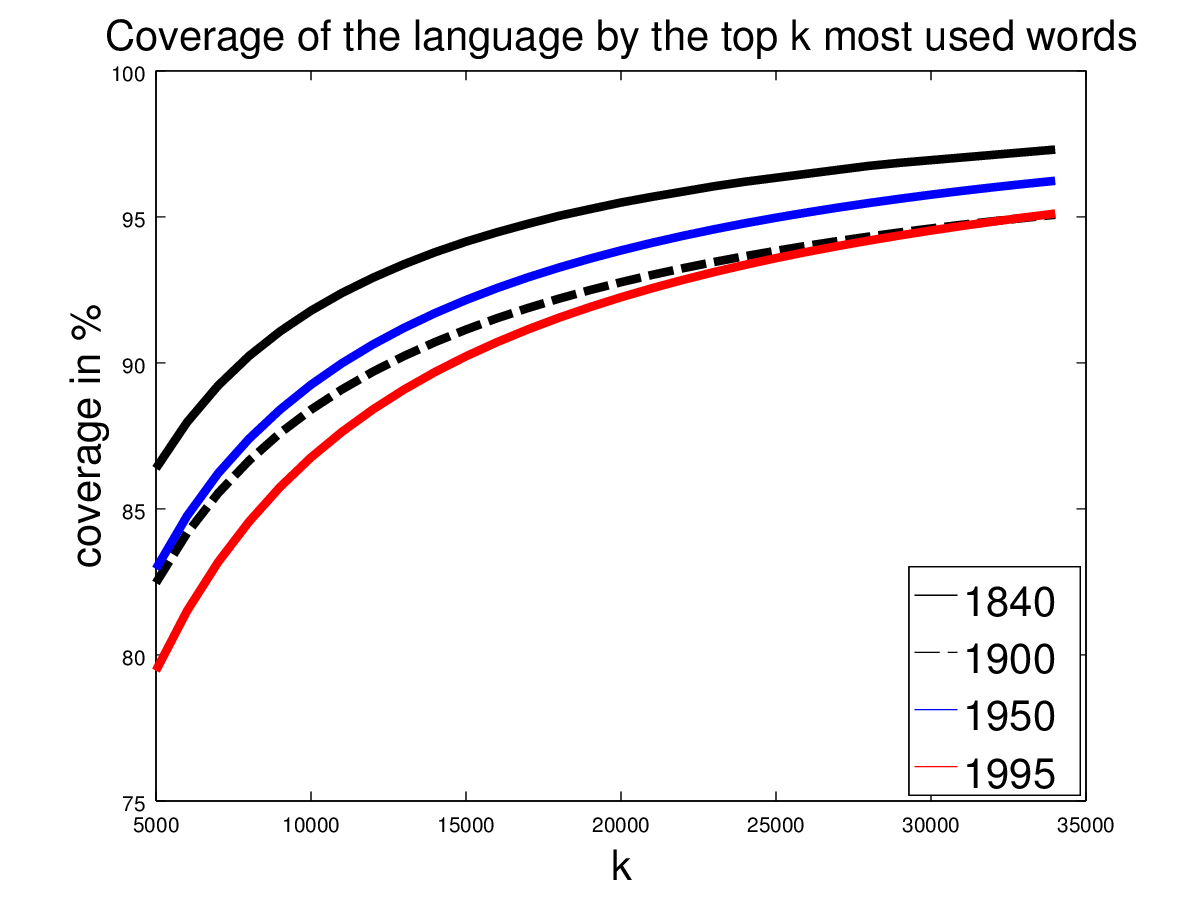
\includegraphics[scale=0.50]{Pictures/statistics/top-k-words-coverage/coverage.png}
    \caption{Percentage of text covered by the top $k$ most used words}
    \label{coverage_figure}
\end{figure}

We can interpret this result in the way that there are more new words than disappearing words, and thus, against our intuition, our everyday vocabulary becomes wider. This can be due to all the vocabulary that appeared with the internet and new technologies.
